%\documentclass[12pt]{article}
%\usepackage[margin=1 in, head=0.9 in]{geometry}
%\usepackage{fancyhdr}
%\usepackage{listings}
%\usepackage{caption}
%\usepackage{color}
%\usepackage{xcolor}
%\usepackage{caption, apacite}
%\DeclareCaptionFont{white}{\color{white}}
%\DeclareCaptionFormat{listing}{\colorbox{gray}{\parbox{\textwidth}{#1#2#3}}}
%\captionsetup[lstlisting]{format=listing,labelfont=white,textfont=white}
%\usepackage{graphicx}
%\usepackage{amsmath, amssymb, amsthm}
%\usepackage[all,cmtip]{xy}
%\pagestyle{fancy}
\input{/home/dmitry/Work/Research/thesis/FINALE/settings.tex}

%\newcommand{\ib}[1]{\bar{#1}}
%\newcommand{\ip}[1]{#1^{\prime}}
%\newcommand{\iti}[1]{\tilde{#1}}
%\newcommand{\pder}[2][]{\frac{\partial #1}{\partial #2}}
%\newcommand{\pderr}[3][]{\frac{\partial^2 #1}{\partial #2 \partial #3}}
%\newcommand{\ap}[1]{\langle #1 \rangle}
%\newcommand{\hx}[2][]{ \hat{#1}_{#2} }
%\newcommand{\hxd}[3][]{ {\hat{#1}_{{#2}_{#3}}} }
%\newcommand{\mb}[1]{\mathbf{#1}}
%\newcommand{\pp}[1]{\partial_{#1}}
%\newcommand{\vphi}{\varphi}
%\newcommand{\hqu}{\mathcal{H}}
%\newcommand{\cj}[1]{{#1}^{\star}}
%\newcommand{\rc}{\operatorname{Re}}	% complex real
%\newcommand{\ic}{\operatorname{Im}}	% complex real
\begin{document}

\title{Gravity wave scattering by large scale sea bottom features}
\maketitle

\section*{Abstract}
The surface and interior wave motions interact with the sea bottom irregularities altering gravity wave energy propagation. Directional scattering and mode conversion will inevitably reshape a wave field and will impel restructure of localized energy budgets. Two geophysically important cases are investigated: (1) a tsunami wave scattering from a prominent sea mount and (2) origination of a semidiurnal internal tide and its reflection    from a continental slope.\\
A tsunami wave is scattered by Koko Guoyt such that amplified and delayed signals were observed during recent tsunami events. The numerical simulations emphasize complicated response. The energy focusing occurs in dependence to tsunami incidence angel and frequencies involved. Koko guoyt as having asymmetrical shape selectively amplifies tsunami waves. The provided theoretical analysis further outlines regions and parameters which would lead to higher amplification.\\
Wave energy can be transported in the ocean's interior by internal waves. E.g., internal tides originate from surface tide interaction with steep submarine ridges. This phenomena undergoes temporal variation leading to nonstationarity in the far field. It is shown for Tasman Sea that remote internal tide modulates magnitude of energy conversion. Further leading to spatial variability many kilometers away.\\
The Tasman Sea internal tides impinge on the continental slope partially reflecting. Efficiency of reflection markedly depends on generation of along slope leaky mode. Under conditions coupling with the surface tide occurs leading to overall energy increase that outgoing energy becomes larger than incident amount. This deviates from classical two dimensional view on reflection/scattering process of the internal tides. The presented estimates of energy transfers further emphasize large variability mainly coming from along slope topography inhomogeneity.\\
Results for both problems conspicuously show importance of three dimensional topographic structure in order to describe wave energy propagation. This has strong effect on variability in the resulting wave field and wave energy sinks.\\
\textbf{INTERNAL PART IS HORRIBLE, too much intro}

\newpage
\section{Introduction}
Oceanic gravity waves fundamentally contribute to redistribution of mechanical energy in the world ocean. The energy pathways of propagating waves can be altered in a result of interaction with large scale sea bottom features such as submarine seamountains, trenches and continental shelves. These processes appreciably shape wave propagation, and thus, leading to variation in the energy budgets. In this work, by means of numerical simulations  energy scattering of tsunamis and internal waves of tidal frequency (internal tides) is examined for cases of their interaction with ocean's bottom relief.\\
Tsunami waves are transient waves impulsively forced by submarine earthquakes and landslides. In the former case their origin lies along oceanic subduction zones such as Japan-Kuril trench (Figure 1a). These waves traversing the Pacific Ocean will encounter numerous sea bottom features. Here let's discuss also energy decay of tsunami waves.\\
These open-ocean scatterers will redirect and delay wave energy creating amplified far-field signals. For example, during the Tohoku tsunami event of March, 11th 2011, tidal gauges in Northern and Central California recorded larger waves than anywhere else along the US West Coast. Notably, for some stations the secondary waves were higher than the primary.\\
Several previous studies have identified that the primary reason for the observed wave distribution is Koko Guoyt. There secondary waves originate as a result of wave scattering. This forms a distinct energy lobe (beam). Its salient feature is a bearing towards the Northern California. Additionally, trapping by Mendocino Escarpment reinforces strong tsunami waves in that region.  As it is seen, generation of the scattered waves have important consequences for forecasting of tsunami wave arrival times and post-event assessment of damage to coastal communities. This work sets its goal to develop a description for scattering mechanism at Koko Guyot.\\
% In this example, delayed waves correlated to a beam of high energy originating from a distant scatterer in Emperor seamount chain, Koko Guyot (Figure 1a). 
\begin{figure}
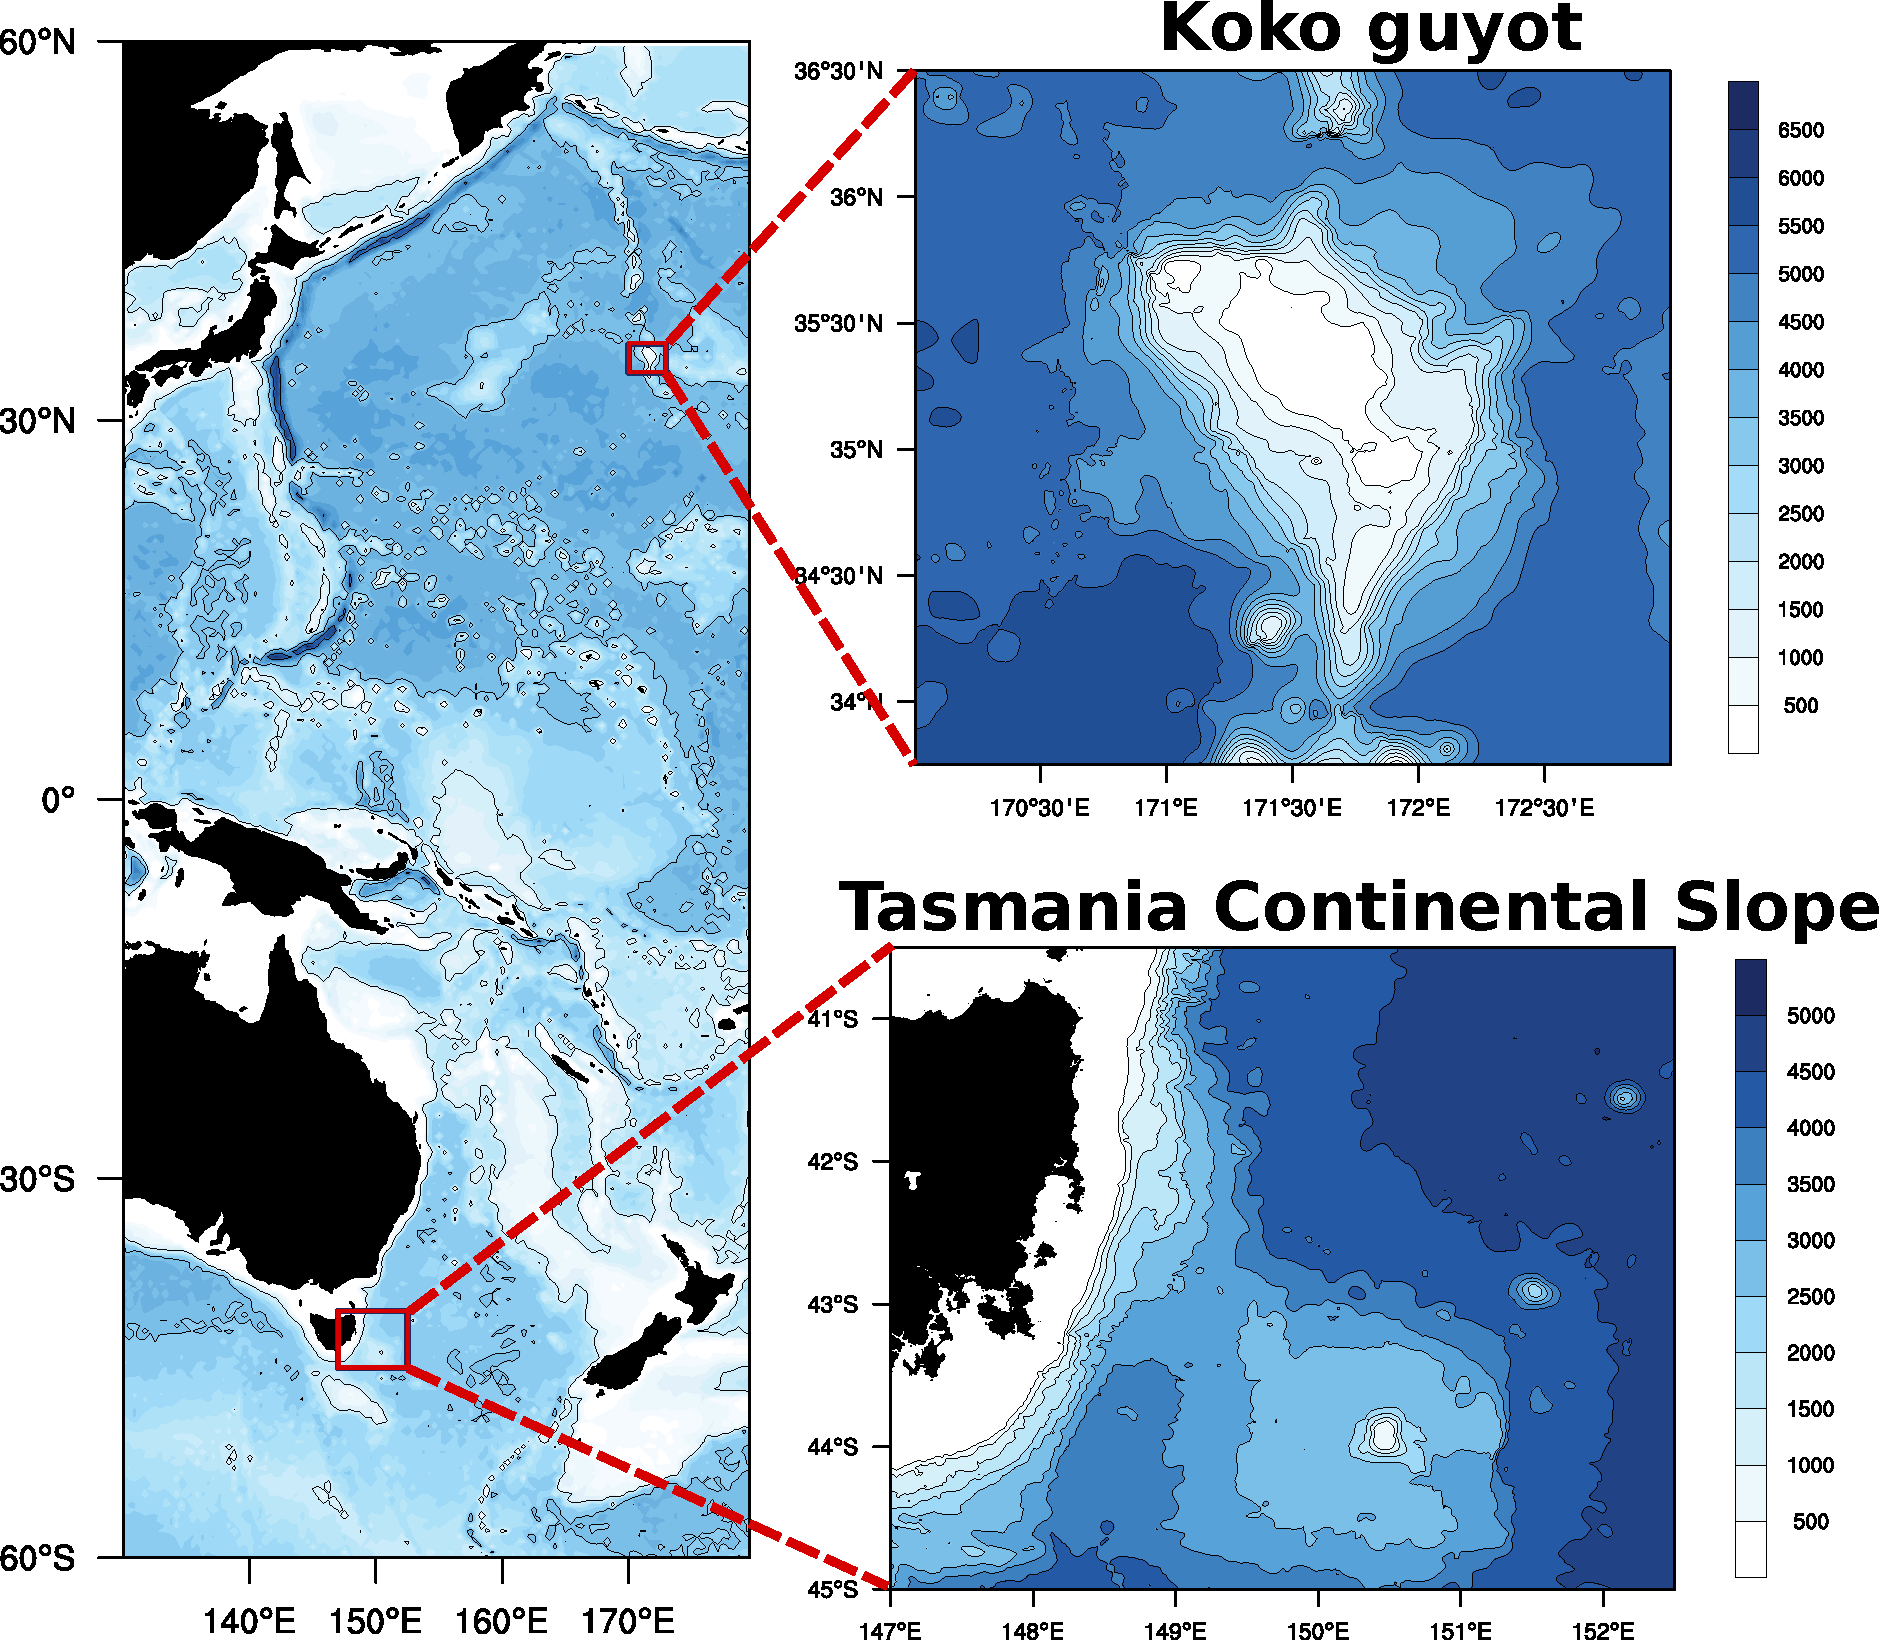
\includegraphics[scale=0.5]{../figures/map_w_places.pdf}
\caption{The map of the Pacific Ocean with outlined regions.}
\end{figure}
Wave phenomena exists through out all water column so that ocean's interior is filled with internal waves. Their existence owns to vertical stratification since the internal waves  travel as an oscillatory motion of isopycnal surfaces. The initial perturbation can be forced by many mechanisms: wind forcing, surface buoyancy forcing, ice keels, etc. Here internal waves are caused by a tidal flow making existence of internal tides. These baroclinic waves are of tidal or quasi-tidal frequency which makes them easy to investigate.\\
The major reason for study of baroclinic tides is their non negligible role in dissipation of barotropic, surface tidal energy. Current estimates suggest that 1/3 of total tidal energy is being converted into internal motions directly in the deep ocean. Further, roughly 1/3 of that energy is lost to turbulent mixing right at generation sites while the rest emitted as freely propagating waves. These waves were observed to cross the ocean basins in form of tight beams (``spider web") without much attenuation. These observations fueled scientific research to simply understand where and how these internal tidal energy is deposited. Since this occurs deep below direct wind influence, the internal tides are thought as one of candidates for providing energy to close upwelling branch of Meridional overturning circulation.\\
In any case, internal tides propagation characteristic and scattering properties are still poorly understand and quantified. This is a goal for Tasman Tidal Dissipation Experiment (TTIDE). Their phenomena to investigate was a scattering of internal tidal beam that crosses Tasman Sea and impinges on continental slope of Tasmania (Figure 1). The primary problem is quantifying how much energy is being reflected into the open ocean. This problem was studied by means of numerous numerical experiments. One of the major concerns presented here is a variability associated with incidence of the tidal beam, intrinsic interactions with topography and background conditions. The description of this mechanisms are useful for description of field observations and consequently creating large scale understanding of internal tide reflection which allows for more describing effects of internal tides on the World Ocean.\\
Both of the investigated geophysical problem represent a type of wave scattering by inhomogeneity in the media. The latter here means rapid change in ocean depth that creating conditions for wave's propagation and energetic characteristics change. As title of thesis implies the problems are dealt by application of energy considerations, mainly energy flux.\\
At such location the energy would drain into perturbations of isopycnals that further can travel hundreds of  leagues without any significant loss of energy. In the second part of my thesis origination, propagation and dissipation of the internal tidal beam is investigated on the example of Tasman Sea. \\
A global internal tide model, satellite altimetry measurements and in situ observations indicate that a ridge south of New Zealand is a site for the generation of the strong tidal beam that is directed towards the Tasman Shelf break. The low mode internal wave beam undergoes scattering from topography, which transfers energy to shorter length scales. Thus, understanding of local energy processes will lead to a more detailed picture of tidal energy dissipation.\\
\textbf{PLUGIN: 2 TW, 1 TW, Macquarie Ridge, internal tides produce transport of particulates: sediments and can cause strong currents in deep ocean. Role in tidal dissipation, Internal tides what became apparent recently are important energy transporters.}
\subsection{Energy conservation and energy flux}
Even though tsunami being surface waves and internal tides are waves traveling on isopycnal surfaces they posses a similarity which enables similar treatment of their energy properties. For both cases the waves are predominantly long, their typical wavelength is much larger than the ocean's mean depth with periods longer than buoyancy period. Both tsunami and internal tides have scales of 200 km. This provides unified description by means of Laplace tidal equations on f-plane with allowance for density stratification (\cite{kundu2008fluid}, \cite{cushman2011introduction}) (or Shallow Gravity waves) which formulated as follows
\begin{align}
\pder[u]{t} - f v = -\frac{1}{\ib{\rho}_0}\pder[p]{x}\\
\pder[v]{t} + f u = -\frac{1}{\ib{\rho}_0}\pder[p]{y}\\
0 = -\pder[p]{z} - \rho g\\
N^2 w = -\frac{1}{\ib{\rho}_0} \pderr[p]{z}{t}\\
\pder[u]{x} + \pder[v]{y} + \pder[w]{z} = 0
\end{align}
with $(u,~v,~w)$ being velocity along zonal, meridional and vertical axis, $f$ - Coriolis parameter, $p$ - perturbation pressure rising from sea level or isopycnal motions of stratified water column given by Brunt-Vaisala frequency $N^2 = -\frac{g}{\ib{\rho}_0}\pder[\rho_0]{z}$. The set of equations is constructed for linear and hydrostatic flow under Boussinesq approximation. Additionally, boundary conditions are imposed on the surface (linearized) and flat bottom,
\begin{align}
w|_{z = 0} = \pder[\zeta]{t},~p|_{z = 0} = \ib{\rho}_0 g \zeta\\
w|_{z = -H} = 0
\end{align}
Such formulated problem allows separation of vertical axis by employing vertical mode decomposition,
\begin{align}
(u, v, p)(x,y,z,t) = \sum_{n = 0} [u_n(x,y,t), v_n(x,y,t), p_n(x,y,t)]\psi_n(z)\\
w(x,y,z,t) = \sum_{n = 0} [w_n(x,y,t)] \int_{-H}^z \psi_n(z) dz\\
\rho(x,y,z,t) = \sum_{n = 0} [\rho_n(x,y,t)] \frac{d \psi_n(z)}{dz}
\end{align}
Upon substitution of the decompositions Sturm-Liouville problem is obtained for vertical structure (basis) functions $\psi_n(z)$,
%\pder[\frac{1}{N^2 - \omega^2} \pder[\psi_n]{z}]{z} + \big(1 - \frac{f^2}{\omega^2} \big) \frac{\psi_n}{c^2_n} = 0
\begin{equation}
\frac{d}{dz}\big( \frac{1}{N^2} \frac{d \psi_n}{dz} \big) + \frac{1}{c^2_n}\psi_n = 0
\end{equation}
with $c_n$ being an eigenvalue for a respective $n$-th mode.\\
The carried out vertical decomposition effectively decouples vertical dynamics from horizontal reducing the initial set to shallow water-type of equations,
\begin{align}
\pder[\vec{u}_n]{t} + f \vec{k} \times \vec{u}_n = -\frac{1}{\rho_0} \nabla p_n\\
\frac{1}{\rho_0} \pder[p_n]{t} + g D_n \nabla  \cdot \vec{u}_n = 0
\end{align}
Here I intentionally introduced equivalent depth $D_n,~c_n = \sqrt{g D_n}$. For typical oceanic conditions $0$-th mode represents a barotropic solution with $\psi_0 = const$, i.e.  vertically uniform dynamics, and $D_0 \simeq H$ (\cite{hendershott1981long}. So it resembles pure surface wave propagation such as tsunami wave propagation. The left out infinite sequence of vertical modes are purely internal modes that cause isopycnal displacements of magnitude, $\eta_n = \int w dt = \int w_n \int_H^z \psi_n dz$ and negligibly small sea level motions. The latter allows complete separation between barotropic and baroclinic (vertically dependent) motions.\\
For tsunami waves due to their high frequency rotational effects are usually neglected, but can appear over long distances (Kowalik, Sumatra). Internal tides on the other hand are Sverdrup waves which are the same as long shallow water waves but perturbed with rotation causing them to be dispersive.\\
This set enables to provide a plane wave solution described with
\begin{align}
\label{In:svw}
\begin{split}
p_n = p_{0n} e^{i \omega t - \vec{k} \cdot \vec{x}}\\
u_n = \frac{1}{\rho_0} \frac{-\omega k_x + i f k_y}{\omega^2 - f^2} p_n\\
v_n = \frac{1}{\rho_0} \frac{-\omega k_y - i f k_x}{\omega^2 - f^2} p_n
\end{split}
\end{align}
so that wave associated current is related to pressure by polarization relations.\\
Now using framework (12-13) energy equation can be formed by multiplying momentum equations with $\vec{u}_n$ and continuity equation with $p_n$ adding both expressions and depth integrating (\cite{nekrasov1990energy}, \cite{kowalik2013oceanography}, \cite{kelly2012cascade}),
\begin{equation}
(E_k + E_p)_t + \nabla \cdot \vec{F} = D \label{In:eneq}
\end{equation}
Additionally, depth averaging is carried out so that energy flux will be defined,
\begin{equation}
\vec{F}_n = \frac{1}{H} \vec{u_n}^(t) p_n(t) \int_{-H}^0 \psi^2(z) dz \label{In:fldef}
\end{equation}
For tsunami wave propagation due to their barotropic phenomena $\psi(z) = 1$ and $p_n = \rho_0 g \eta$, the energy flux comes to its classical form for surface wave propagation, \cite{kowalik2013oceanography}, $\vec{F} = \rho_0 g \vec{u} \zeta$. I deliberately abandon nonlinearity terms presuming deep ocean propagation. Koko Guoyt depth on average is around 500 m, barotropic velocity is of order $0.1~m/s$, nonlinear terms scale as $\sim u^3$, while linear energy flux as $\sim g u \zeta$. It suggests that only in shallow water where horizontal acceleration is of order of gravity acceleration, nonlinear terms will be a significant addition to total energy transports.\\
In internal tidal studies I additionally carry out period averaging due to harmonic character of waves which is given by Euler formula, $(u,v,p) \sim e^{i \omega t}$, so that (\ref{In:fldef}) becomes
\begin{align}
\vec{F}_n = \frac{1}{2} \cj{\vec{u}}_n p_n \int_{-H}^0 \psi^2(z) dz
\end{align}
The same discussion on nonlinear additions stays true for internal tide scattering from the Tasman continental slope which depth does not exceed $100~m$. Only on shallow shelfs advection of kinetic energy becomes non-negligible (\cite{kang2012energetics}, \cite{nash2012unpredictable}).\\
Energy conservation, \ref{In:eneq} sets an useful framework for analysis of the wave interaction with topography. As bottom slope starts rapidly change, wave propagation undergoes variation resulting in reorientation of currents, divergence of water column. But because of energy conservation (under assumption of nonfrictional flow), amount of total energy should be preserved. Hence, transports of energy through control volumes can present a valuable tool for description of wave interaction with bottom relief. The assumption of nonfrictional flow does not fully hold in the problems considered, but dissipation is not considered in this thesis because of its not primary reason. So that any inconsistencies in control volume calculations are said to be due to either dissipation (both physical and numerical) and due to errors in analysis.\\
After normal mode framework was formulated it is instructional to consider how well it is hold. For tsunami wave this check can be easily done by comparison of Airy wave dispersion (\cite{kundu2008fluid}) with long wave approximation (Figure 2). It is of no surprise that on top Koko Guoyt and on its walls the tsunami break limit for shallow water approximation, so that assumption on flat bottom breaks and validity of the presented dynamics is under suspicion.\\
For internal tides application of normal mode analysis is invalid since for sloping bottom full threedimensional structure should be considered. This would lead to a hyperbolic equation which lands a wave propagation along characteristics (\cite{sandstrom1969effect}) or internal wave beams. their direction are set by the buoyancy frequency,
\begin{equation}
\gamma = \frac{dz}{dx} = \pm \frac{\omega^2 - f^2}{N^2 - \omega^2}
\end{equation}
In case of bottom slope exceeding characteristics angle, $\nabla H > \gamma$ internal waves are reflected (\textit{supercritical regime}), while less inclined topographies there is a forward propagation (\textit{subcritical regime}). The analytical solution for internal wave propagation on sloping bottom was worked out previously (\cite{wunsch1968propagation}, \cite{wunsch1969progressive}) can be compared with normal mode fitting (Figure 3). This  establishes that for internal tide interaction with supercritical continental slope the normal mode approach fails. 

\begin{figure}
\mfig[0.5]{tsunami_regimes.pdf}
\caption{Tsunami regime propagation. Shallow water limit vs deep water limit}
%\includegraphics[scale=0.5]{../}
\end{figure}

\begin{figure}
\mfig[0.8]{errors2.pdf}
\caption{Internal wave propagation on slope in nonrotating, uniformly stratified ocean with inclined bottom.}
%\includegraphics[scale=0.5]{../}
\end{figure}
Nevertheless away from inclined topography normal modes is a successful approach in understanding how wave energetics changes upon interaction with the prominent bottom relief. So what actually happens when the wave encounters bottom slope? Wave scattering.

\subsection{Formulation of scattering problem}
In the previous section the normal mode approach was formulated under condition of flat bottom. This produces a simplified boundary condition $w|_{z = -H} = 0$ which further enables variable separation. Thence, vertical motions became decoupled from the horizontal variability. As wave encounters sloping bottom the boundary condition does not hold any more and becomes fully nonlinear,
\begin{equation}
\vec{u} \cdot \nabla h = 0 \label{In:bcnon}
\end{equation}
Now the boundary condition clearly states that there is no mass transport across impermeable bottom as wave impinges. Wave itself cannot satisfy (\ref{In:bcnon}), hence, additional motions should arise such that the total mass transport will be zero across the boundary. In the most simplistic configuration when a wall is placed against incident wave train, a specular reflection will occur in order to satisfy (\ref{In:bcnon}). Hence, the reflected wave is ``generated" or this can be restated as an incident wave was scattered into a reflected one. To additionally emphasize this point, here and forth wave scattering is a process of wave generation in order to satisfy of no mass transport across ocean's bottom.\\
By now considering a step-like discontinuity in ocean depth the so-called matching conditions can be devised (\cite{mei1989theory}) from (\ref{In:bcnon}) and continuity equation for scattering of surface gravity waves,
\begin{align*}
\vec{u}_1 h_1 = \vec{u}_2 h_2,~\zeta_1 = \zeta_2
\end{align*}
which restates the previous point and additionally emphasizes continuity of sea level. The same approach is also used in studies of internal tide scattering (\cite{larsen1969internal}, \cite{chapman1981scattering}) and internal tide generation problems (\cite{st2002role}). But with a separated condition of no flow through a barrier. In actuality, internal tide production can be viewed as scattering of surface, barotropic tide by steep bottom relief (\cite{hendershott1981long}). Internal tide scattering produce not only change of direction such as for surface waves, but also energy leakage into other vertical modes. MORE ON INTERNAL TIDE SCATTERING Griffith\& Grimshaw.\\
Of additional note, in rotating ocean the boundary condition has the same form, but physically, due to elliptic particle motions in Sverdrup wave \eqref{In:svw}, a coupling occurs between zonal and meridional current components \cite{greenspan1968theory}.\\
From energetic point of view as wave scattering occurs portion of the inicident energy is transfered into other wave motions. For tsunami wave this can be characterized by differential scattering cross section (\cite{landau1988hydrodynamics}) defined as an amount of energy emerged in some differential direction $(\theta, \theta + d \theta)$.\\
In internal tide studies it is of more importance to indentify energy transports from the incident field into other modes (\cite{kurapov2003m}, \cite{kelly2012cascade}. Such that
\begin{align}
C_{n}^{bt-bc} = w_{bt} \cdot p_n\\
C_{mn}^{bc-bc} = (\cj{\vec{u}}_m p_n \int_{-H}^0 \psi_m \nabla \psi_n dz - \cj{\vec{u}}_n p_m \int_{-H}^0 \psi_n \nabla \psi_m dz)
\end{align}
In these two expressions it is explicitly made a separation between transfer from baroptropic tide into internal tidal mode $n$. And in the second energy transfer from internal tidal mode-$n$ to mode-$m$.\\
As scattering occurs, no one can guarantee that incident wave will preserve its form and its energy. So that, for example, a barotropic Sverdrup wave will transfer partially its energy into Kelvin wave (\cite{pinsent1972kelvin}). Or that scattered waves will be free. Trapping of wave energy is a well known phenomena (\cite{longuet1967trapping}, \cite{kowalik2002tidal}).\\
Since in this work energy approached is considered, it is advisable to formulate scattering problem in terms of wave energetics. Aforementioned, scattered waves are generated from the incident wave field, so there is a direct energy transfer which is controlled by \eqref{In:bcnon}. Let consider a system of reference moving with an incident wave. Than the boundary condition will simply postulate of scattered field generation. This can be transferred into an energetics. The boundary surface will hence doing of work on scattered field. So that emitted energy flux is given by,
\begin{equation}
F_{sc} = p_{sc} u_{sc}
\end{equation}
It can be shown (\cite{morse1958theoretical})	that it will have angular distribution in far from the scatter, so differential scattering cross-section can thus introduced.\\
If angular distribution 
 \\

Generally speaking, wave scattering happens due to inconsistency of boundary conditions. This can be expressed as the following equation.\\

Internal tide generation was ascribed to scattering of barotropic tidal energy from bottom relief.

\newpage
\section{TO DO}
\begin{itemize}
\item In my writing here I need to write down energy conservation equation. It must be done super careful. Ref: Wunsch, Ferrari; Nekrasov; 
\item Definition of energy flux since it is corner stone for the whole work. Ref: Kowalik papers; Nash, Kelly

\end{itemize}

\bibliographystyle{apacite}
\bibliography{/home/dmitry/Bibtex_lib/my_first_lib}

\end{document}